%% entwurf.tex
%% $Id: entwurf.tex 28 2007-01-18 16:31:32Z bless $
%%

\chapter{Entwurf}
\label{ch:Entwurf}
%% ==============================

Für das Aufzeichnen, der für die Studie relevanten Daten wird eine auf dem Smartphone der Probandin installierte Android Applikation benötigt. 
Dieses Kapitel beschäftigt sich mit dem Entwurf dieses App und setzt sich mit dem Zugriff verschiedener Datenquellen auseinander.
Eine grobe Skizze des Systems ist in Abbildung \ref{skizze} zu sehen.
Der Entwurf soll darauf abzielen, der Nutzerin möglichst wenig aufzufallen, um ihr Verhalten nicht zu beeinflussen.
Das Ziel soll sein, keinerlei Interaktion abgesehen von der Installation und dem Export der Daten zu benötigen. 
\par

Die App zur Studie wurde für Geräte mit mindestens Android 5.0 "`Lollipop"', das entspricht dem API Level 21, entworfen.
Das heißt, dass aufgrund der Rückwärtskompabilität auch alle neueren Geräte in der Lage sind die Applikation auszuführen.
\par

%%Die Entscheidung als Minimal API Level 21 zu wählen geht war notwendig, da mit diesem die UsageStatManager Schnittstelle für Applikationen zum Android Betriebssystem hinzugefügt wurde.
%%Von anderen Aspekten der Applikation benötigte API Levels waren:

Die Entwurfsentscheidung über das zu nutzende API Level ist immer eine Abwägung;
Auf der einen Seite steht das niedrigere API Level, das wie im Kapitel \ref{ch:Grundlagen} beschrieben, 
eine breitere Menge an potenziellen Testprobandinnen eröffnet.
Andererseits haben höhere API Level oft viele Verbesserungen und neue Schnittstellen mit denen Entwickler mehr Funktionalität erreichen können.
\par
Die Entscheidung für das relativ aktuelle API Level 21 ist auch davon motiviert , 
% dass der potenzielle Pool von Testprobandinnen im Umfeld der Informatik oft über aktuellere Smartphones und Android Versionen verfügt
dass mit Level 21 einige Neuerungen im Bereich der Aufzeichnung von Applikationsaktivität hinzugefügt wurden.

Untermauert wird dies von der bereits im vorangehenden Kapitel vorgestellten Statistik \ref{fig:androidplatformdistr}  von Google\cite{androiddistr}, 
die Android 5.0 "`Lollipop"' mit 36.1\% als die meistgenutzte Version des Android Betriebssystems.

\par

%TODO: Systemskizze.
\begin{figure}[h]
    \centering
    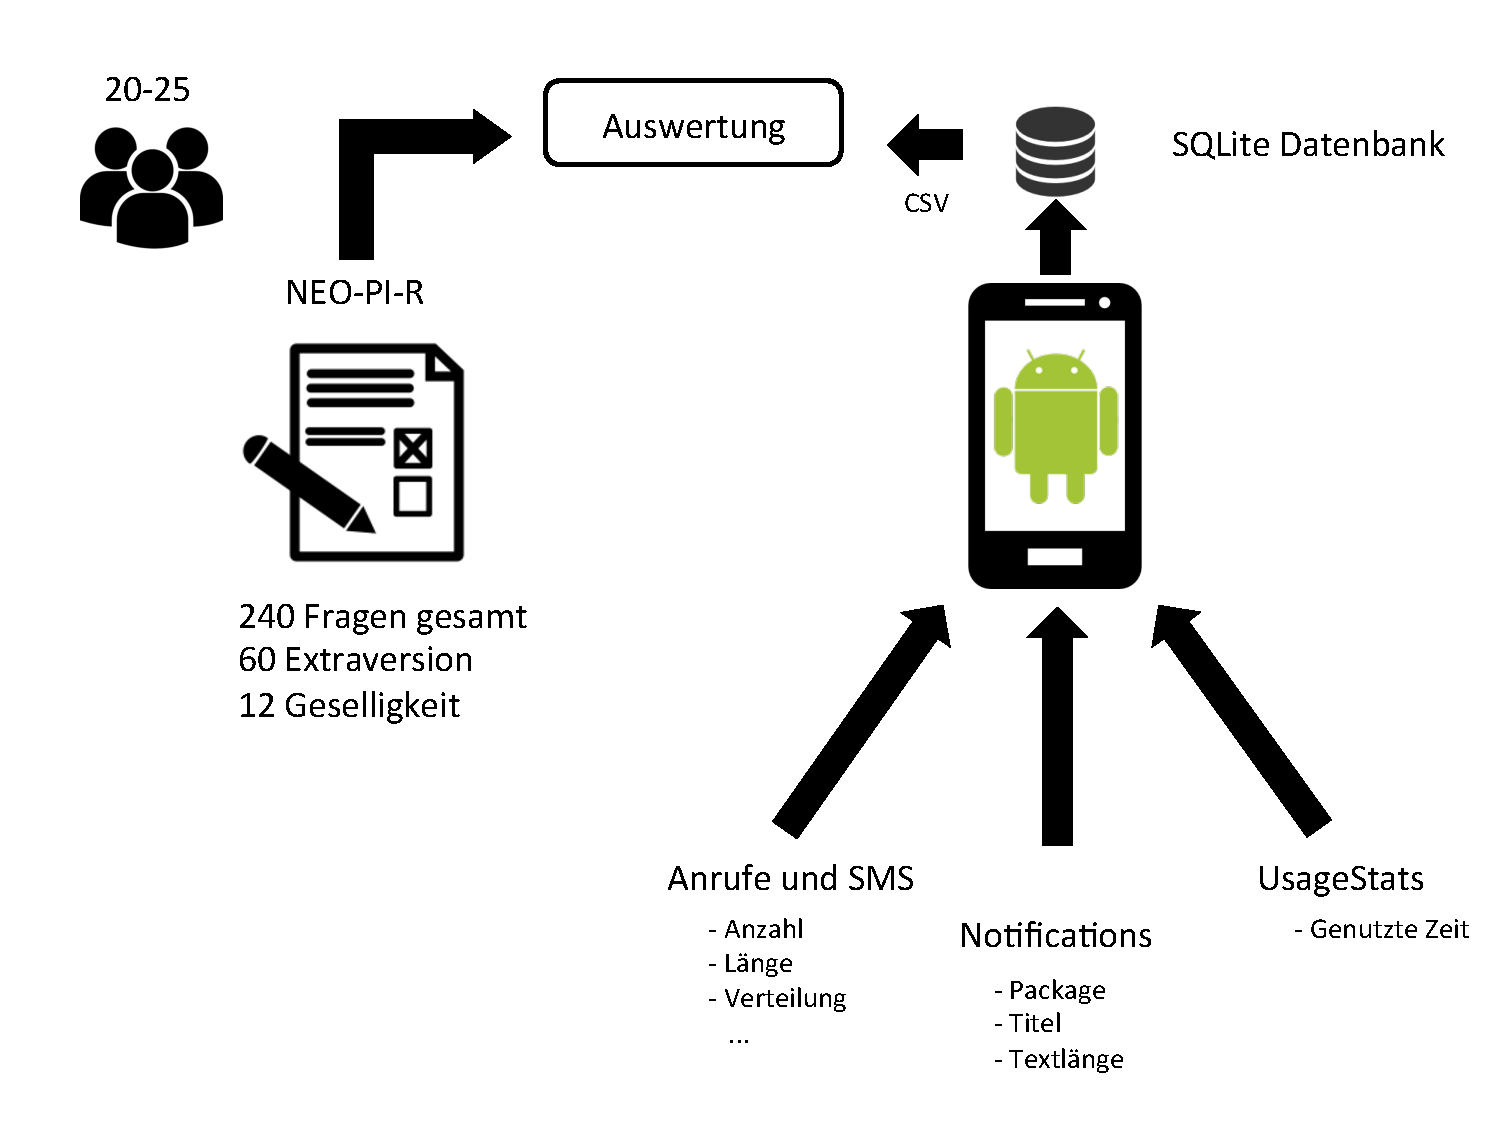
\includegraphics[width=\textwidth]{images/skizze.pdf}
    \caption{Systemskizze}
    \label{skizze}
\end{figure}


\section{Datenquellen}

%Das Nutzungsverhalten der Studienteilnehmerinnen soll mit einer Android Applikation aufgezeichnet werden.
%Die Applikation soll mit so wenig Nutzerinteraktion wie möglich auskommen.
Für das Aufzeichnen des Nutzerverhaltens werden drei beziehungsweise vier verschiedene Datenquellen betrachtet.
\par

\subsection{Call und Message Log}
Zunächst werden die konventionellen Kommunikationsmöglichkeiten eines normalen Mobiltelefons betrachtet.
Daten zu Anrufen und Kurznachrichten (SMS) lassen sich in Android mit Zugang zum \emph{Call Log} und zum \emph{Message Log} auslesen.
Die Berechtigungen dafür können von der Nutzerin bei der Installation erteilt werden und müssen nicht nocheinmal bestätigt werden.
Für das Sammeln dieser Daten muss nicht aktiv das Verhalten der Nutzerin geloggt werden und es muss auch keine Datenbank dazu angelegt werden,
da das Android Betriebssystem dies bereits erledigt.
Es genügt beim finalen Abgeben der Daten auf die Call und Message Logs zuzugreifen und die relevanten Daten auszulesen, da man den Abfragezeitraum beliebig wählen kann.
Um ein aussagekräftiges Ergebniss zu erhalten ist die Wahl der relevanten Daten, die untersucht werden, von entscheidender Bedeutung. 
Aus diesem Grund wurden für diese Arbeit verschiedene Ansätze der Wahl der zu betrachtenden Features in Betracht gezogen. 
Dabei verspricht der Ansatz aus \cite{chittaranjan2011s} für unsere Zwecke auf Grund seiner breiten Fächerung die besten Resultate.
\par

%\subsection{Call Log}
Dementsprechend wurden folgende für diese Arbeit interessanten Features aus dem Call Log extrahiert:

\begin{itemize}
    \item Anzahl Anrufe gesamt
    \begin{itemize}
        \item Anzahl Anrufe ausgehend
        \item Anzahl Anrufe eingehend
        \item Anzahl Anrufe verpasst
    \end{itemize}

    \item Anrufdauer gesamt
    \begin{itemize}
        \item Dauer Anrufe ausgehend gesamt
        \item Dauer Anrufe eingehend gesamt
    \end{itemize}

    \item Durschnittliche Dauer gesamt
    \begin{itemize}
        \item Durchnittliche Dauer Anrufe ausgehend
        \item Durchnittliche Dauer Anrufe eingehend
    \end{itemize}

    \item Unique Anrufpartner
    \item Maximale Anzahl Anrufe mit einem Partner

\end{itemize}

%\subsection{Message Log}
Analog zum Call Log wurden folgende Features aus dem Message Log extrahiert:

\begin{itemize}
    \item Anzahl SMS gesamt
    \begin{itemize}
        \item Anzahl SMS gesendet
        \item Anzahl SMS empfangen
    \end{itemize}

    \item SMS Zeichenanzahl gesamt
    \begin{itemize}
        \item SMS Zeichenanzahl gesendet gesamt
        \item SMS Zeichenanzahl empfangen gesamt
    \end{itemize}

    \item Durchschnittliche SMS Zeichenanzahl gesamt
    \begin{itemize}
        \item Durchschnittliche SMS Zeichenanzahl gesendet
        \item Durchschnittliche SMS Zeichenanzahl empfangen
    \end{itemize}

\end{itemize}


\subsection{Notifications}


\ignore{todo: refereces}
Über den im Grundlagenkapitel bereits vorgestellten NotificationManager, beziehungsweise einen NotificationListenerService, kann auf dem Gerät der Nutzerin eine SQLite Datenbank angelegt werden,
in die alle während dem Studienzeitraum der Nutzerin gezeigten Notifications gespeichert werden.
Die Spalten der SQLite Datenbank sind die Folgenden:
\begin{description}
    \item ["`\_id"'] fortlaufende Indentifikationsnummer
    \item ["`notificationEntry"'] Package der Applikation von der die Notification gepostet wurde
    \item ["`titleHashed"'] Gehashter Titel der Notification, Bei Nachrichten oft der Absender
    \item ["`textLength"'] Anzahl Zeichen im Text der Notification
    \item ["`date"'] Zeitpunkt, an dem die Notification gepostet wurde
\end{description}

Im Sinne des Schutzes der Privatsphäre beinhalten diese Einträge nicht exakt den Inhalt der Notification, sondern so anonymisiert, dass die für die Studie relevante Information erhalten bleibt.
So wird der Titel der Notification mit dem SHA-1 Hash\cite{sha1def} gehasht.
SHA-1 ist eine 1995 von US Amerikanischen Nachrichtendienst NSA veröffentlichte kryptographische Hashfunktion\cite{sha1proposal}.
Dies führt dazu, dass für die Auswertung der Studie zwar zwischen zwei verschiedenen Absendern von Nachrichten unterschieden werden kann, diese aber nicht frei zu erkennen sind.
Ebenso speichert die Applikation für die Studie nur die Länge der erhaltenen Nachrichten und nicht deren Inhalt, da dies ein sehr schwerwiegender Eingriff in die Privatssphäre wäre.
Der Zeitpunkt wird im Datenformat Millisekunden seit Epoch angegeben.


\subsection{UsageStats}

Über den im Android API Level 21 eingeführten UsageStatsManager ist es möglich 
auf die vom Android Betriebssystem selbst gesammelten Daten bezüglich der Zeit aller Applikationen im Vordergrund zuzugreifen.


TODO: MEhr UsageStats + Auswahl App + Statistik

\subsection{Auswahl Applikationen}

Alle verwendeten Apps aller Probandinnen zu betrachten und im Hinblick auf ihre Signifikanz bezüglich der Geselligkeit festzustellen würde den Rahmen einer Bachelorarbeit überschreiten.
Außerdem wäre dies ein größerer Eingriff in die Privatsphäre der Probandin als notwendig.
Deshalb wurde sich auf eine bestimmte Menge von Applikationen begrenzt, deren Notifications und UsageStats gesammelt werden sollen.

%Um vom Umfang der Arbeit im Rahmen einer Bachelorarbeit zu bleiben und gleichzeitig nicht einen größeren Eingriff in die Privatsphäre der Probandin als nötig zu tätigen,

Hierzu wurden folgende Applikationen ausgewählt:
\begin{description}
  \item [Google Hangouts] Crossplattform Kommunikationsdienst von Google. Auf aktuellen Android Smartphones vorinstalliert.
  \item [Whatsapp] Crossplattform Instant Messaging Client. Mit über einer Milliarde Nutzer die meistgenutzte Messaging Application\cite{whatsappuser}.
  \item [Facebook App] Mobile Applikation des größten und aktivsten Social Networks mit über einer Milliarde aktiver Nutzer pro Tag\cite{facebookuser}.
  \item [Facebook Messenger] Dedizierte Messenger Applikation von Facebook.
  \item [Skype] Dedizierte VoIP und Messaging Applikation zu Microsofts Skype mit über 600 Millionen Nutzern\cite{skypeuser}.
  \item [Telegram] Crossplattform Kommunikationsdienst, das sich durch verschiedene Sicherheitsoptionen von seiner Konkurrenz abhebt. Über 100 Millionen Nutzer\cite{telegramuser}.
  \item [Twitter] Social Microblogging Service mit 300 Millionen aktiven Nutzern. Aufgrund der offenen API gibt es verschiedene Twitter Apps, von denen die größten betrachtet werden:
  \begin{itemize}
      \item Offizielle Twitter App
      \item Carbon for Twitter
      \item Plume for Twitter
      \item Talon for Twitter
  \end{itemize}
\end{description}




%% ==============================
\section{Zusammenfassung}
%% ==============================
\label{ch:Entwurf:sec:zusammenfassung}

Die Studie, die im Rahmen dieser Arbeit durchgeführt wird, untersucht zwei Datenpunkte.
Zum einen die von der Applikation gesammelten Daten zum Nutzungsverhalten von zehn bestimmten Social Media und Instant Messaging Applikationen
und zum anderen die zu der Nutzerin zugeordneten Extraversions-, beziehungsweise Geselligkeitswerte aus einem Persönlichkeitstest.
Als für das Einschätzen des Nutzerverhaltens relevante Smartphonedaten wurde einerseits die Häufigkeit, Länge und Verteilung von  Anrufen und SMS bewertet,
als auch die Notifications und UsageStat von zehn Kommunikations- und Social Media Applikationen.
Dabei wird besonderes Augenmerk auf den Schutz der Privatsphäre der Nutzerin und deren Daten gelegt.
Bis auf das Ausfüllen des Persönlichkeitstests, dem Aufsetzen der Applikation und dem Exportieren der Daten am Ende der Studie sollen die Nutzerinnen nicht weiter belastet werden.


%%% Local Variables: 
%%% mode: latex
%%% TeX-master: "diplarb"
%%% End: 
